%%
%%                  TEMPLATE for Math 404 project report
%%
\documentclass[11pt]{amsart}
%%% WARNING: Do NOT change the page size, fonts, or margins!  Penalties will apply.


\usepackage{graphicx}
\usepackage{amssymb,amsmath,amsthm}
\usepackage{mathrsfs}
\usepackage{placeins} %enables \FloatBarrier, which prevents figures and tables from going below it.
\usepackage{hyperref} %makes cross references into hyperlinks. 
\usepackage{caption}
\usepackage{subcaption} %Allows subfigures
 

%%% WARNING: Do NOT change the page size, fonts, or margins!  Penalties will apply.
%%% WARNING: Do NOT change the page size, fonts, or margins!  Penalties will apply.

\title{The Cost of Living: A Zillow Housing Forecast}
\author{Patrick Beal, Tiara Eddington, Madelyn Vines}

% Change the date to match the date you actually wrote this paper
\date{\today} % or use \today




\begin{document}

\maketitle % this actually makes the title

\begin{abstract}
The purpose of this paper is to provide a method for forecasting changes in housing market trends on multiple levels.
We include data on median income, taxation, house price, and demographic breakdown, each at a state level.
Our analysis includes K-means time-series clustering, ARIMA system forecasting, and Bayesian hierarchical modeling.
We hypothesize that using these methods, we can predict future housing market trends (assuming no shocks) and make inferences about the factors influencing shifts in the market. The source code associated with this project is available in the GitHub \href{https://github.com/jpatrickb/vol3_housing_project}{Housing Project Repository}.

% Every day buyers and sellers struggle to make real estate decisions. It is difficult to know where the housing market will move in the future, where to buy/sell, and when to buy/sell. We hope to make these decisions easier by forecasting future housing prices and showing general trends by region.

% Place abstract here. The abstract summarizes in one paragraph the main question, results, and conclusions drawn from your investigation.  
\end{abstract}

%% First Section
\section{Problem Statement and Motivation}
Housing prices play a critical role in shaping household wealth, investment strategies, and public policy.
Understanding their drivers and future trajectories is essential for buyers, sellers, policymakers, and researchers alike. 
This study models housing price dynamics from 2000 to 2020 using a combination of demographic data and regional features to improve prediction accuracy and provide insight into regional housing market behavior.

We pursue two primary purposes: (1) to determine regions with similar housing market behavior, aiding investors in portfolio diversification; and (2) to forecast future housing prices using historical and demographic predictors.
We use prediction and inference to provide useful information about housing markets to answer these questions.
Along with helping investors identify where to invest, these results help potential homeowners and policymakers understand the factors that influence market growth.

% One question a buyer or seller might be asking is: What state is best to move to given my financial situation and goals? We hope to identify sstate with low price intercepts and high slope. This indicates that you are buying at a low price relative to how much the home will grow in value, making the profits greater if you sell later on. Another question is: If I am interested in investing in real estate, what regions should I buy houses in order to diversify my real estate assets? Ideally, we will be able to group states that are similar in housing markets so that buyers can pick houses in diverse groups. Finally, real estate buyers or sellers will want to know: What will future housing prices be in a given area based on prior information? We suspect that characteristics such as location, race, and trends in previous housing prices will be strong features in predicting future prices. 

Previous research on housing price prediction has applied various machine learning techniques.
For example, while Random Forests tend to be highly accurate during training, they are also prone to overfitting.
In contrast, gradient boosting models such as XGBoost and LightGBM generalize more accurately, and Hybrid Regression approaches can improve accuracy by combining multiple models, though they are less computationally efficient \cite{TRUONG2020433}. 
Another study employed data mining and linear regression to analyze historical market trends and forecast future housing prices \cite{Bhagat2016}. 
Additional research has explored economic models such as supply-demand frameworks and hedonic regression, incorporating factors like immigration, urbanization, fertility rates, and life expectancy.
Studies found that such factors explain approximately 40\% of the observed increase in housing prices between 1970 and 2010 \cite{GONG2022103734}. 

% Suggested future work includes: investigating the coupling affect and finding faster training methods. % I commented this line out because I don't think we need it, it really doesn't fit with any of our analysis - Patrick
The approach we take includes examining the impacts of demographic factors on the housing market, along with more traditional approaches looking only at housing data.
We apply a broader range of models and include models specifically tailored for time series analysis, including VARMAX, auto-ARIMA, and Bayesian hierarchical modeling, using clusters by states.
 

%%Second Section
\section{Data} 
% Zillow data:
% - Downloaded state-level housing prices on the last day of each month from January 2000 to January 2025
%   - Median house price
% - Removed unnecessary information, such as region type, size rank, region ID
% - Some states had no data at the beginning of the time, so we just used the first value

% CPS Data:
% - Current population survey (give description)
% - Includes household level observations, with data on location (state and county), income, property tax, number of people in the household, marital status of parents, race, and population weight
%    - Using weights, we found average income, property tax, proportions of each race, and population for each state and kept only those values
% - Missing values were a result of not having any samples to contribute to a given mean, which only occurred in population values. We filled these with zeros
% - Limitations: This survey is conducted on a subsample of the population, so the estimates are not completely representative of the true distributions of each value for each state

% Merging:
% - Linear interpolation of all the CPS data to be along the same time index as the Zillow data
%    - Linear interpolation makes more sense than holding values constant and changing once per year, since values such as population and proportion of race change gradually
% - Merged with housing data on the date and state index
\subsection{Sources}
We use two primary data sources.
First, for house prices, we use Zillow's Home Price Index (HPI) which contains state-level median home prices for each month from January 2000 to the current~\cite{zillow}.
For demographic, tax, and income data, we use the Current Population Survey (CPS), a yearly survey administered to a subset of the population by the U.S. Census Bureau.
To obtain the variables listed from this dataset, we use the Integrated Public Use Microdata Series (IPUMS) data tool~\cite{IPUMS_CPS_2024}.

\subsection{Cleaning}
The housing data was mostly complete, with missing values following two patterns: (1) seemingly random, isolated points missing from the data, and (2) missing data at the beginning of the time period, presumably before data was collected for a given state.
These missing values affected very little of our data, with North Dakota being the only state that had several years of missing values at the start of the time period, and a very small portion missing randomly throughout the dataset.
For the points missing completely at random, we linearly interpolated between the month before and the month after for the state with the missing value.
Similarly, in the case of North Dakota, where we miss several years of data at the beginning, we just filled the missing values with the first value present.
This assumption is clearly wrong, as we know that the housing prices were not constant for several years, though we have no way of knowing the true HPI for those years. We added a column to our dataframe with flags indicating whether we had filled in missing data so that we could take this into account in our modeling and analysis.
% The data was mostly complete, but we had to address a few cases of missing values. 
% For missing data points that occurred in the middle of the time series, we used linear interpolation method to estimate values based on surrounding data. These instances were very few and isolated, so interpolating based on the data immediately preceding and following the missing point did not cause any changes in the overall trend.
% In cases where data for some states started later and were missing entire years from the beginning of the dataframe, we filled in the missing early values with the first available measurement and added a flag to indicate these fills and added a column for each region to indicate whether leading data was filled in and for how long. Only a few states had this issue, so by adding a flag we were able to keep track of these and be wary of the results produced from modeling these states' data.
% Lastly, we removed identifying information unnecessary for analysis, only keeping the states, years, and housing price index.

% We also merged demographic data from the Current Population Survey (CPS), provided by the Integrated Public Use Microdata Series (IPUMS) \cite{IPUMS_CPS_2024}.
% The CPS, sponsored by the U.S. Census Bureau and the Bureau of Labor Statistics, offers household-level data on location, income, property tax, family structure, and race.
% IPUMS
In the CPS data collected from IPUMS, we faced much larger issues with the data.
Because the survey is based on a small sample of the population, the proportions of each race are not perfectly representative of the true populations in each state.
For example, most states reported having no people for many of the race combination categories, so these values were essentially useless.
Rather than trying to fill these missing values, we simply dropped them, considering only White, Black, Asian, and Native American (Note: Hispanic is considered an ethnicity, so this was not included in racial data).
Also, because the CPS is administered yearly, we chose to perform a linear interpolation to estimate race proportions in each month so that the CPS data follows the same time scale as the Zillow data.
We chose linear interpolation rather then simply repeating each value twelve times because it is more likely that the racial proportions changed gradually throughout the year than very quickly at the beginning of a new year.

We then merged the housing and demographic data on the month and state.
Because of the market shock of the COVID-19 pandemic from which our economy is still recovering, we chose to only use the data up to January 2020 (further justification for this is given in Section 4.2).
Altogether, this gave us a dataset containing HPI, demographic proportions, median income, and median property tax in 51 states (including the District of Columbia) across 241 total months.
We chose to perform an 80-20 test split, using up to January 2016 as training data, and from February 2016-January 2020 as testing data to evaluate the forecasting power of our model. Because our entire test set occurs after the training data chronologically, we avoid any leakage of testing information into our training set.

% To merge the datasets, we linearly interpolated the CPS data to match the monthly time points of the Zillow data. 
% Linear interpolation makes more sense than holding values constant and changing once per year, since values such as population and proportion of race change gradually. The merged dataset, covering 51 states and 301 months, includes both housing prices and demographic characteristics. Due to the COVID-19 pandemic in 2020, the housing prices experienced a drastic shock that makes training and forecasting very difficult. As a result, we choose to drop data after January 2020. We divide the data into training (up to 2016) and testing (2016-2020) sets, 80\% an 20\% train-test split, maintaining chronological independence between the two.


% Discuss the sources, reliability, and suitability of your data for the problems you are addressing.  The dataset should be large enough and rich enough to give reliable, meaningful, and nuanced answers to the questions and problems addressed in your project. Remember that test-train-validation splits for sequential and time-series data are trickier than for tabular data. Be clear about how you handled splitting data into test, training and validation sets, and how you ensured that there was no leakage between test and training set and no other similar data problems.  Be clear about how you handled missing data.  Justify your choices on all these things. 

%% Third Section
\section{Methods} 
 

\subsection{Time-Series K-means Clustering}
We clustered the various states according to the observed changes in housing prices, using \texttt{Time-} \texttt{SeriesKMeans} from \texttt{sklearn.clustering}. This tool allows us to use \texttt{KMeans} to cluster, but with an algorithm designed specifically for time series data.
This gives clusters of states that tend to grow in similar ways, allowing us to perform further analysis on the aggregation of states within each cluster.

\subsection{Classical Decomposition}
To begin analyzing our data, we tested different detrending methods. We attempted to detrend via differencing, moving average, and OLS to find the method that produced a nearly covariance stationary time series. 
We found that differencing gave the best results, and we used this method throughout our modeling. % TODO: More explanation here?
We then analyzed the different components of our time series using a classical decomposition. we approximated the trend and season with a 12-month period using the \texttt{statsmodels.tsa.seasonal} package.
We assumed that housing prices have a roughly yearly seasonal period, based on the idea that people are more likely to move during different times of year \cite{seasonal}.
After detrending our data, we used time series analysis methods to understand which models give the best forecasts of future housing prices.

\subsection{Autoregressive Integrated Moving Average}
First, we tried fitting models on housing price data for individual states using the \texttt{auto\_arima} model from \texttt{pmdarima}.
For this model, we tested orders of autoregression and moving averages up to a maximum of 12, assuming that each data point should at most depend on the values from the entire previous year.
Next, we attempted to forecast housing data based on information about other variables, such as housing data from other states with a similar housing market or with the state's own demographic data. We trained and evaluated \texttt{VARMAX} models to analyze both of these effects.

\subsection{Bayesian Hierarchical Model}
Finally, we created a Bayesian hierarchical model to make inferences about the influences on the data and to provide an alternative method of predicting future time series values.
We used a linear parameter model with hierarchical parameters allowing for unique intercepts and time slopes for each state.
Let $P$ represent the median house price, $tax$ be the average property tax, $pop$ be the population, $\alpha_{native}, \alpha_{asian}, \alpha_{black}$, and $\alpha_{white}$ be the proportion of the population in each racial category.
Our hierarchical model considers state-level parameters for the time slope and intercept, drawing from a population distribution, as well as population parameters for the coefficients on tax, population, and race data.
Further, we let $i$ denote the state and $t$ denote the time (in months).
Our estimated linear model is
\begin{align*}
    P_{i, t} &= \beta_i^0 + \beta_i^t \ t + \beta_{tax}\ tax_i + \beta_{pop}\ pop_i + \beta_{native}\ \alpha_{native, i}  \\
    & \qquad + \beta_{asian} \alpha_{asian, i} + \beta_{black}\alpha_{black, i} + \beta_{white} \alpha_{white, i} + \epsilon, 
\end{align*}
with the prior distributions
\begin{align*}
    \beta_i^0 & \sim \mathscr{N}(\mu, \sigma_{\mu}), 
    &\beta_i^t  \sim \mathscr N(\eta, \sigma_{\eta}), \\
    \beta_{tax} & \sim \mathscr N (0, 20), 
    &\beta_{pop}  \sim \mathscr N (0, 1), \\
    \beta_{native} & \sim \mathscr N (0, 10{,}000), 
    &\beta_{asian}  \sim \mathscr N (0, 10{,}000), \\
    \beta_{black} & \sim \mathscr N (0, 10{,}000), 
    &\beta_{white}  \sim \mathscr N (0, 10{,}000), \\
    \epsilon & \sim \mathscr N(0, \sigma), 
    &\mu \sim \mathscr N(200{,}000, 100{,}000), \\
    \eta &\sim \mathscr N(1{,}000, 1{,}000), 
    &\sigma \sim \text{HalfCauchy}(100). \\
    \sigma_{\eta} &\sim \text{Exp} \left(\frac{1}{5{,}000}\right), 
    &\sigma_{\mu} \sim \text{Exp}\left(\frac{1}{50{,}000}\right), \\
\end{align*}
We select mean-zero with narrow variance for the tax and population coefficients because these values can change a lot, though we don't anticipate huge changes in the house price as a result (relative to the size of the change in these values).
The population coefficient prior distributions were chosen with large variance and mean zero because the proportion of the population in each race is very small, so it changes very little, though we allow for large changes in the median house price as a result of these changes.
For our hyperparameters $\mu$ and $\eta$, we select rough estimates as the means with large variances so as to allow the model to explore and converge to the right population values.
Next, $\sigma_{\mu}$ and $\sigma_{\eta}$ were selected to have exponential distribution with very wide tails to avoid imposing too tight of a prior distribution on the variance of our prior distribution.
We chose the exponential distribution rather than Half Cauchy because using Half Cauchy was actually found to not be restrictive enough and prevented the sampling from converging.

Before sampling, we first use $z$-score normalization mapping $x_{i, t}$ to $\frac{x_{i, t} - \overline{x}_i}{\sigma_i}$ to transform the independent variables and standardize the scales to allow for easier sampling.
Because of this normalization, the interpretation on our coefficients is the effect of a one-unit change in standard deviation in a feature on the housing price.
The interested reader can refer to Figure~\ref{fig:ppd} of the Appendix, which shows that the prior predictive distribution is not too restrictive of the data and thus should allow the sampler to converge well, though the prior does not cling tightly to the distribution of the data.


% Your project should involve a thoughtful and original use of several of the machine learning methods and ideas we have learned in class and at least one idea or method we have not covered in class.  
% In this section you should describe and justify your selection of models, your choices of methods, any feature engineering you did, and the ways and reasons you chose your hyperparameters or network architectures.   Your discussion should demonstrate a clear understanding of the principles involved and of the strengths and weaknesses of the models and methods used.  



%%Fourth Section
\section{Results and Analysis}

\subsection{Time-Series K-means Clustering}

% If someone wants to diversify their investments, they should consider buying houses in diverse markets. We decided to use time series clustering to show which states are most similar to each other. Our KMeans algorithm was trained on the percentage change in housing prices and predicted with 2-10 clusters. We found that the states consistently grouped together those in the middle. As we increased the number of clusters the middle region group shrunk \ref{fig:Cluster3}, \ref{fig:Cluster7}. We found similar results when clustering on demographic features. This result indicates that if you want the most diverse real estate investment, in terms of percent change in housing price, then you might want to buy houses in a mixture of middle states and states along the perimeter of the country. States like California and Florida often were clustered either by themselves or in the smallest groups, making them seem to have a more likely difference than other states.
% If someone wants to diversify their investments, they should consider buying houses in diverse markets. To explore this, we used time series clustering to identify which states have similar housing price trends. Our KMeans algorithm was trained on the percentage change in housing prices from 2000 to 2020 and run with 2 to 10 clusters. We found that states in the geographic center of the country consistently grouped together, while coastal states like California and Florida often formed their own smaller clusters (see Figures~\ref{fig:Cluster3} and~\ref{fig:Cluster7}). As the number of clusters increased, the central region group gradually shrank. We found similar patterns when clustering on demographic features. This suggests that, for investors seeking diverse real estate portfolios in terms of housing price changes, it may be beneficial to buy properties in a mix of central states and states along the perimeter of the country.

To aid real estate investors seeking diversification, we applied time series clustering to identify groups of states with similar housing price dynamics. Using KMeans clustering on the percentage change in housing prices from 2000 to 2020, we evaluated solutions with 2 to 20 clusters. Across specifications, states in the geographic center of the country tended to cluster together, while coastal states such as California and Florida often formed distinct, smaller clusters (see Figures~\ref{fig:Cluster3} and~\ref{fig:Cluster7}).

As the number of clusters increased, the central region group became increasingly fragmented, suggesting greater heterogeneity among mid-range markets. A similar pattern emerged when clustering on demographic features, reinforcing the relationship between regional housing trends and population composition. These results imply that to maximize geographic diversification in real estate investment—measured in terms of differentiated housing price trends—investors should consider combining properties from both central and peripheral states.

When using more than seven clusters, the amount of clusters that have only one state increases, thus isolating outliers rather than revealing meaningful groupings.
This suggests that the returns to using higher numbers of clusters are diminishing, so limiting the number of clusters used to at most will give the most useful results in diversifying investments.
Because we are clustering by housing price growth and not any geographical features, the clustered states are are not necessarily neighbors.

% From 7 clusters on, the percentage of clusters with one state per group increases from 10\% to 50\%. Because of this, we would not recommend using more than 7 clusters. If you want to buy N houses, you should approximately buy 1 in each of the N clusters, unless N is greater than 7. In this case, you should start to buy a few in each group, as long as they are sufficiently spread between clusters. One weakness of this method is that if your purchasing decisions are not based on housing prices or demographics then the clusters may not diversify in the desired way.

\begin{figure}[h]
    \centering
    \begin{subfigure}{0.45\textwidth}
        \centering
        \includegraphics[width=\linewidth]{figures/3clusters.png}
        \caption{}
        \label{fig:Cluster3}
    \end{subfigure}
    \hfill
    \begin{subfigure}{0.45\textwidth}
        \centering
        \includegraphics[width=\linewidth]{figures/7clusters.png}
        \caption{}
        \label{fig:Cluster7}
    \end{subfigure}
    \caption{US states clustered into 3 (A) and 7 (B) clusters (Note that the clusters are based on housing price growth, not location).}
    \label{fig:clusters}
\end{figure}

\subsection{Classical Decomposition}
The most interesting result of applying a classical decomposition to our data set was that the seasonal component of housing prices in each state had two different peaks throughout the year.
Though the height of each peak varied from state to state, nearly every state displayed housing prices that peak halfway through the year, decrease for one to three months, then increase and peak again before the end of the year.
Additionally, the classical decomposition led us to believe that housing markets over the past five years are associated with a different trend and seasonal component than in prior decades.
This conclusion comes from the observation that the residual component of the housing data for each state is relatively small %TODO: more info on 'relatively' small?
from 2000 to 2019, but starting in 2020, the residual plot becomes erratic and fluctuates rapidly, with a much larger magnitude than previous years (see Fig. \ref{fig:utah deomposition}).
This makes sense, because housing prices are subject to random shocks that are heavily dependent on the country's overall economic conditions, as well as changes in economic policy.
The start of the COVID-19 pandemic in 2020 drastically affected both of these features, providing a plausible explanation for the variation in housing prices after 2020.
However, this change makes training and forecasting after 2020 based on data from before 2020 very difficult, which is why we choose to only include pre-2020 data for prediction and forecasting, as mentioned earlier.

\begin{figure}[htbp]
    \centering
        \centering
        \includegraphics[width=4in]{figures/utah_prices.png}
        \caption{Housing Prices in Utah, 2000-2024}
        \label{fig:utah deomposition}

\end{figure}



\subsection{Autoregressive Integrated Moving Average}
\subsubsection{Univariate ARIMA}

We used a variety of ARIMA models in an attempt to forecast future housing prices.
First, we used the \texttt{auto\_arima} model to determine the optimal order of difference, number of autoregressors, and order of the moving average component for an ARIMA$(p, d, q)$ model.
We allowed the model to grid search over values $1 \leq p, q, \leq 12$, and to find the parameters that minimize the model's AIC. We found the optimal model to be an ARIMA(4, 1, 0) model, the results of which are shown in Fig.~\ref{fig:ohio forecast}, \ref{fig:utah forecast}. 
Because we hypothesized that housing prices would be very prone to random shocks, it is surprising that the optimal model does not have a moving average component, and this presents a potential topic for further study.
The main issue we encountered when forecasting with ARIMA models is that the forecast accuracy differs significantly across states.
The optimal model seems to forecast an approximately linear trend that continues along the same slope as the most recent training data.
Some states do actually follow this trend, but the ARIMA model doesn't do a good job of accounting for changes in trends due to shocks.
After training models on every state, only 30 out of 51 models produced forecasts that captured the true testing data within the 95\% confidence interval.
This metric could also be problematic because the variance of the predictions increases as the forecast continues.
For some states, the variance becomes so large that the forecast is almost trivial because the 95\% confidence interval spans hundreds of thousands of dollars. %should we include another plot to show this?

\begin{figure}[h]
    \centering
    \begin{subfigure}{0.45\textwidth}
        \centering
        \includegraphics[width=\linewidth]{figures/utah_forecast.png}
        \caption{}
        \label{fig:utah forecast}
    \end{subfigure}
    \hfill
    \begin{subfigure}{0.45\textwidth}
        \centering
        \includegraphics[width=\linewidth]{figures/ohio_forecast.png}
        \caption{}
        \label{fig:ohio forecast}
    \end{subfigure}
    \caption{ARIMA Forecasting on Housing Prices in Utah (A) and Ohio (B), 2000-2020}
    \label{fig:utah and ohio forecast}
\end{figure}


% \begin{figure}[htbp]
%     \centering
%     \begin{minipage}{0.45\textwidth}
%         \centering
%         \includegraphics[width=2.5in]{figures/utah_forecast.png}
%         \caption{Forecasting Housing Prices in Utah, 2000-2020}
%         \label{fig:utah forecast}
%     \end{minipage}\hfill
%     \begin{minipage}{0.45\textwidth}
%         \centering
%         \includegraphics[width=2.5in]{figures/ohio_forecast.png}
%         \caption{Forecasting Housing Prices in Ohio, 2000-2020}
%         \label{fig:ohio forecast}
%     \end{minipage}
% \end{figure}

\subsubsection{Vector ARIMA}

We also experimented with forecasting future housing prices using \texttt{VARMAX} models.
We hypothesized that the housing price in one state can be more accurately predicted using information about other states with similar housing markets.
We used time series clustering to partition the 50 states into 7 clusters based on the percent change in housing price.
For each cluster, we initialized and trained a \texttt{VARMAX} model using housing data for each state assigned to that cluster (see Fig. \ref{fig:utah varmax}).
In many cases, these models provided more accurate forecasting than univariate ARIMA.
The \texttt{VARMAX} models did a better job of forecasting fluctuation in the trends of housing prices, as opposed to the roughly linear trends forecasted by \texttt{auto\_arima}.
It is important to note that this method is not useful in all cases, because clustering algorithm placed some states in singleton clusters, with no related states to include in combined model.
For states belonging to a non-trivial cluster, this model seems to give more reliable forecasts than univariate ARIMA, but for states that do not belong to a cluster, there is no indication that either model is better than the other.
We also trained \texttt{VARMAX} models on individual states' data for both housing price and demographic features, hoping that the correlation between housing prices and social and racial demographics would result in more accurate forecasting. Unfortunately, these models did not yield good results.
For many states, the model completely failed to converge and predicted a constant housing price equal to the mean of the time series.
For a few states, the model converged and gave usable results, but these cases were scarce and there did not appear to be any discerning feature between the states for which the model did not converge and the states for which it did.

\begin{figure}[htbp]
    \centering
        \centering
        \includegraphics[width=4in]{figures/utah_varmax.png}
        \caption{\texttt{VARMAX} Forecasting on Housing Prices in Utah Based on Market Clustering, 2000-2020}
        \label{fig:utah varmax}

\end{figure}


\subsection{Bayesian Hierarchical Model}
To estimate the parameters in the hierarchical model described earlier, we apply the No-U-Turn (NUTs) algorithm, implemented in PyMC3.
This algorithm is an extension of the Hamiltonian Monte Carlo Sampling algorithm, which improves sampling efficiency.
We ran four chains, each tuning with 2000 samples, then iterating for 2000 more samples, obtaining 8000 samples in total for each parameter.
% As with the other models, this model was only trained on the data up through 2016.

Figure~\ref{fig:trace_plot} in the appendix shows the trace plot resulting from the sampling, including the overall distributions for the intercept $\mu$ and slope $\eta$, along with posterior distributions for the slope and intercept for each state, and the stope for the standardized features.
The results give reason to believe that the distributions of parameters have converged, with overlapping kernel density estimates of each parameter and erratic plots of the samples, showing that the sampling algorithm did not get stuck in a tail of the distribution.

The strength of the hierarchical model is shown in Figure~\ref{fig:intercept_forest} and Figure~\ref{fig:slope_forest}.
We see the mean and a 94\% credible interval for the posterior distributions of the slope and intercept parameters for each state, indicating which states had the highest prices in 2000 which have been growing fastest since then.
From these, we observe that Washington, D.C. and Hawaii have been growing the fastest, while Nevada and Michigan have been growing the slowest (or even decreasing on average, from 2000 to 2016).

Although the basic form of the model is a linear regression, because of the unit standardization performed before running the model, the interpretations of the coefficients are ambiguous.
However, because each feature now has the same scale, we can interpret the magnitude of the coefficients as the importance of this feature relative to the other features.
For example, an increase in the native American population tends to lead to a decrease in housing prices, as shown in Figure~\ref{fig:trace_plot}.


% Clearly and succinctly describe your results. Give a thorough analysis and a thoughtful discussion of the conclusions that can be drawn.  Discuss the suitability and effectiveness of the different models and methods for the problems or questions treated.  


%%Fifth Section
\section{Ethical Implications and Conclusions}
We did not identify any privacy issues with the collected data, as it was aggregated by region and did not reveal any information about individuals. However, there are still important ethical issues to consider. One concern is the use of demographic features, such as race, in our predictions. If factors like race or other potentially biased characteristics influence the model's predictions, it could imply that living in areas with certain racial compositions may affect housing prices for buyers or sellers. This could perpetuate bias or lead to unfair treatment.

Additionally, labeling certain states as having more favorable housing trends may lead to a rush of people moving there, which could skew our results and make them less accurate. This could potentially create a harmful feedback loop, where regions with higher proportions of certain racial groups are perceived as less desirable places to live. This could discourage people from moving to those areas or purchasing homes, stunting the region's development and making it even less appealing.

Aside from racial concerns, our findings on housing market correlations and real estate portfolio diversification could be valuable to real estate developers or wealthy investors seeking to increase their passive income. However, this could also lead to wealthier individuals or companies buying up properties in developing markets, driving up housing prices and making homes less affordable for average buyers.

Given the ethical concerns and the inconsistency of some of our models, it would likely be unethical to use our results to advise individuals on where to live or purchase homes, or to form opinions about specific regions. A more ethical application of this data would be for policymakers to better understand the factors influencing housing prices and use this information to inform economic policies and allocate funding to regions in need of support.

% Thoughtfully analyze the ethical implications of your research questions, the data you gathered, and the analysis that was performed.  Are there privacy or other implications from the collection or use of the data?  Could your results and methods be misused or misunderstood?  What can and should be done to prevent misuse and misunderstanding?  Could your algorithms and methods result in a destructive self-fulfilling feedback loop?  How could that be prevented or controlled?  What other ethical implications does your work have?  

%% Sixth section
\section{Conclusion} 
The main conclusion from our analysis is that forecasting housing prices is highly challenging. While some models performed better than others, we didn’t find a consistent approach that reliably predicted prices. This is likely due to the volatility of economic conditions, as housing prices are influenced by a variety of random shocks. For example, we saw significant price changes following the 2008 recession and the 2020 COVID-19 pandemic. These events highlight that we lack enough data to capture all factors affecting housing prices. While we identified correlations between race proportions, population, income, and housing prices, other factors like economic policies, political leadership, crime rates, and natural disasters also play significant roles. Further research that incorporates these factors into forecasting models would be valuable.

Although our forecasting was unreliable, we discovered interesting patterns in the distribution of housing prices across the U.S. We expected regional similarities in housing markets (e.g., Midwest, Pacific Northwest), but our clustering analysis revealed two primary clusters of states, with only a few outliers (see Fig. \ref{fig:Cluster3}, \ref{fig:Cluster7}). This was supported by our \texttt{VARMAX} modeling, which showed that forecasting using data from states in the same cluster generally produced better results than using data from just one state.

From the Bayesian model, we found that race, taxation, and population size impact housing prices. Specifically, larger populations of Native Americans, Asians, and whites were associated with lower housing prices (up to 2016), while higher proportions of Black residents were linked to rising housing prices. The hierarchical structure of the model was beneficial for estimating both state-specific and overall parameters, reducing variance in estimates from states with fewer data points. However, the simple linear model used here doesn’t account for market shocks.

Future research will focus on Bayesian hierarchical models that better account for economic shocks. While predicting housing prices remains difficult, methods like ARIMA and Kalman filters can provide occasional insights, though not consistently. The Bayesian approach shows promise for capturing both broad trends and state-specific movements through shrinkage effects. We believe combining autoregressive models with Bayesian hierarchical models will improve accuracy, better account for shocks, and provide a more robust understanding of housing market trends.


% The clearest conclusion we can make from our analysis and modeling of data is that housing prices are very difficult to forecast. Though some methods outperformed others, we did not find a model and set of inputs that reliably produced accurate forecasting results. We attribute this to the volatility of the economic situation in recent years, and the fact that housing prices are largely determined by random shocks that come from a number of different factors. For example, we saw drastic changes in the trend of housing prices across the U.S. surrounding both the recession in 2008 and the beginning of the COVID-19 pandemic in 2020. Because of this, we reasoned that we do not have enough data features to represent all of the inputs that affect housing prices. We did see a correlation between race proportions, population, income, and housing prices, but housing prices are also very likely correlated to things such as national economic policies, political leadership within a certain region, the overall economic condition in the U.S., and even natural disasters. A more thorough dive into the factors involved in housing prices, as well as a further attempt to model and forecast using those factors, would be valuable topic for further research.

% Though our forecasting results were not very reliable, we found interesting results in describing the distribution of housing prices in the U.S. We expected to find that different regions of the U.S. (e.g. the midwest, the New England region, the Pacific northwest), would have similar housing markets within themselves. However, the results of time series clustering showed that the majority of states fall into two main clusters, with the rest of the clusters only containing a handful of outliers (see Fig. \ref{fig:Cluster3}, \ref{fig:Cluster7}). This conclusion is supported by the results of our \texttt{VARMAX} modeling, which showed that for the states that belong to significant clusters (i.e. clusters that contain more than one state), forecasting by considering data from the rest of the states in the cluster produced better results than forecasting solely on one states data.

% From the Bayesian model, we can draw inferences on the impact that race, taxation, and population have on the state housing price.
% We learned that greater populations of native Americans, Asians, and whites tends to lead to lead to decreased housing prices (up to 2016) while a greater proportion of black people leads to increasing housing prices.
% The hierarchical structure provides many benefits, such as effective estimation of both overall population parameters and state-specific parameters as draws from the larger distribution, along with shrinkage to reduce the variance of estimates from states with few samples.
% However, the simple linear model used in this case fails to capture the intricacies of the data and account for shocks to the market.
% Future work will include Bayesian hierarchical estimations of more robust economic models that account for shocks in the market more effectively.

% Overall, we have learned that predicting the future is extremely difficult.
% Various factors within states can complicate the ability to predict.
% Frequentist models such as ARIMA and Kalman filters can sometimes provide meaningful estimates on some states, but not consistently.
% The Bayesian methods show promise for being able to simultaneously capture both large-scale trends and individual state movements through shrinkage effects.
% In future work, we believe that a combination of the autoregressive components and the Bayesian hierarchical model can more effectively and accurately predict market trends, including the effects of shocks, while accounting for the different impacts that the shocks have on different areas as a result of demographic breakdown and other factors, providing a robust and informative posterior distribution for housing market trends.


%All text before this line should end before page 11 starts.
%%%%%%%%%%%%%%%%%%%%%%%%%%%%%%%%%%%%%
%% Bibliography below
%%%%%%%%%%%%%%%%%%%%%%%%%%%%%%%%%%%%%
\FloatBarrier % Keep all figures from being put after the bibliography
\newpage
%% If using bibtex, leave this uncommented
\bibliography{refs} %if using bibtex, call your bibtex file refs.bib
\bibliographystyle{alpha}

%% If not using bibtex, comment out the previous two lines and uncomment those below
%\begin{thebibliography}{99}
%\bibitem{Vandermeersch} First reference goes here
%\end{thebibliography}

\newpage
\section{Appendix}
Here, we include the large plots from the Bayesian model that require their own page.
These should not count towards the page count but are still fun for people who want to see them.

\begin{figure}[hbtp]
        \centering
        \includegraphics[width=0.75\linewidth]{figures/prior_predictive_samples.png}
        \caption{Prior Predictive Distribution}
        \label{fig:ppd}
    \end{figure}

\begin{figure}[hbtp]
        \centering
        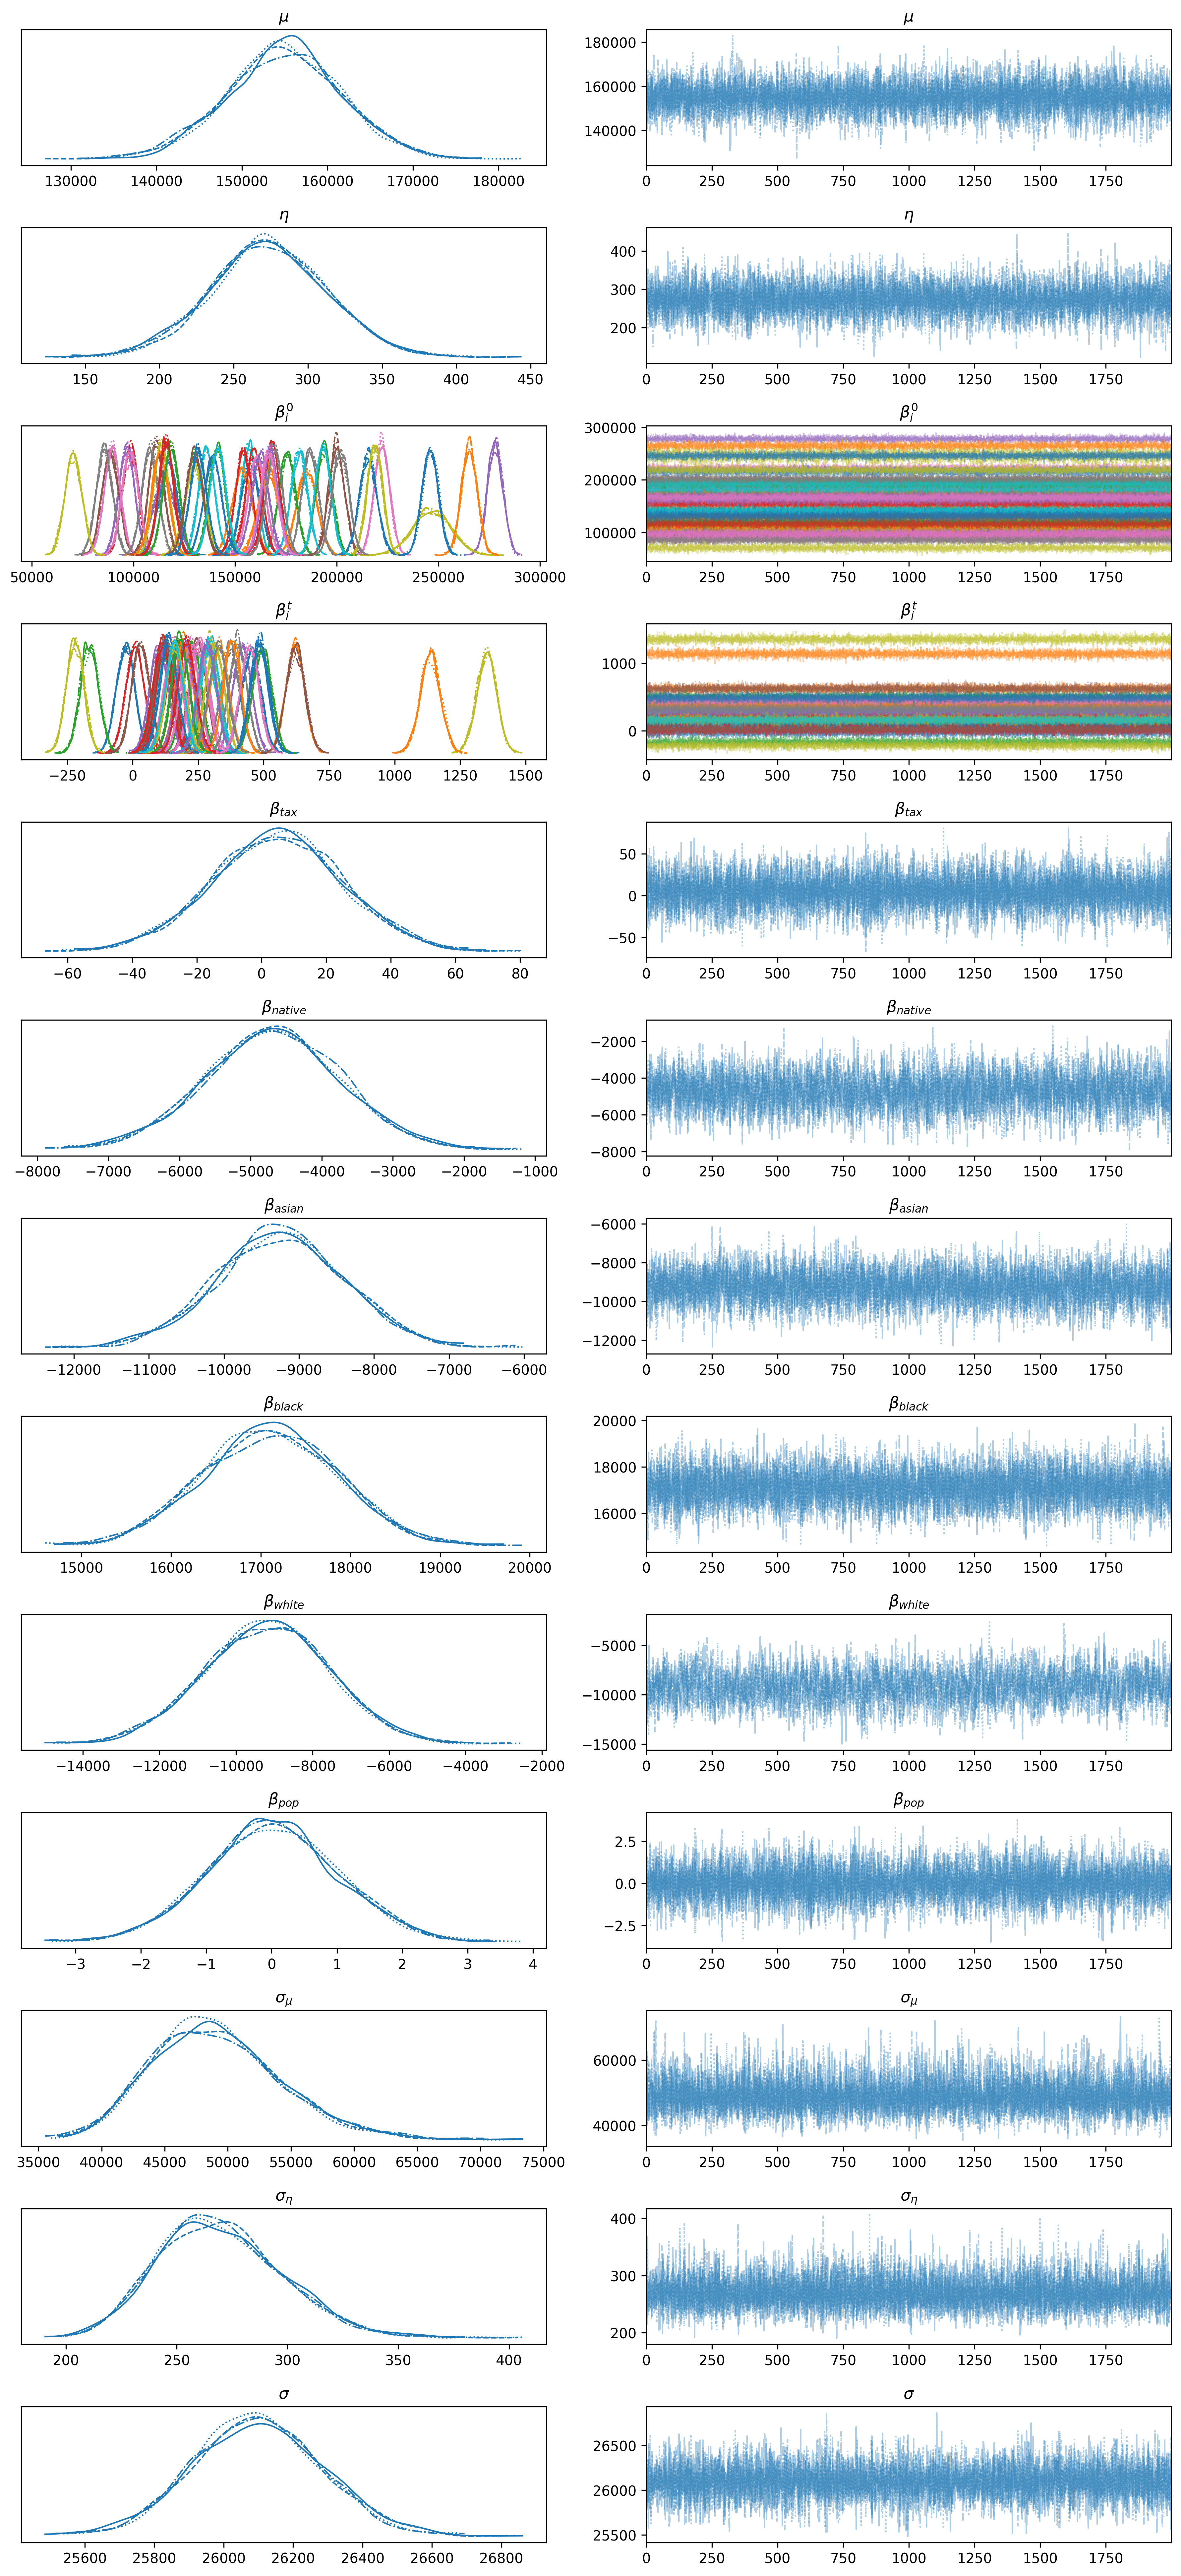
\includegraphics[width=0.75\linewidth]{figures/trace_plot.png}
        \caption{Trace Plot of the Posterior Distributions from Bayesian Estimation}
        \label{fig:trace_plot}
\end{figure}

\begin{figure}[htbp]
    \centering
    \begin{minipage}{0.5\linewidth}
        \centering
        \includegraphics[width=2.5in]{figures/intercept_forst.png}
        \caption{Posterior Distributions on the Intercept for each State}
        \label{fig:intercept_forest}
    \end{minipage}\hfill
    \begin{minipage}{0.5\linewidth}
        \centering
        \includegraphics[width=2.5in]{figures/slope_forest.png}
        \caption{Posterior Distributions on the Slope for each State}
        \label{fig:slope_forest}
    \end{minipage}
\end{figure}

\end{document}
